% einleitung.tex
\chapter{Introduction}
\label{chapter:introduction}



Whether exploring peaceful forest trails on a weekend hike, cruising scenic routes on a bike or embarking on an enjoyable run along riverside paths, many people typically opt for tours tailored to their personal preferences.
Outdoor activities are pursued for leisure and often not meant as a means of transportation from one location to another.
On the contrary, in most cases, roundtrip routes that start and end at the same point are preferred.
For some, these roundtrips mean beginning a run or cycling tour at home and concluding back there. 
For others, returning to the point of departure, where their vehicle is parked, after a hike is necessary.



%Algorithms for shortest paths are an important and much studied part of computer science.
%The topic of finding shortest paths directly influences the lives of many people.
%However, for outdoor activities, the goal might not always be to find the quickest or shortest route.
%Whether someone wants to go running, ride their bicycle, go hiking, skateboarding, inline skating or do any other outdoor activity, in most cases the desired route is a roundtrip rather than the shortest path between two (separate) points.
%Most sports or general outdoor activities are done during free time and are not meant to get from one point to another, but should end at a specified starting point e.g. at home.
%Additionally, if these hobbies involve driving to a park or into an area where the landscape is more fitted to the person's personal goals, finding a good roundtrip of the desired length that brings the person back to their starting point can be especially desirable.
%

Outdoor activities cannot only be fun but also offer many inherent benefits: 
For overall health \cite{oja_health_2011, ruegsegger_health_2018, vina_exercise_2012}, the cardiovascular system \cite{nystoriak_cardiovascular_2018}, as a measure against many different diseases \cite{oja_health_2011}, and for social \cite{mueller_jogging_2007, obrien_jogging_2007, wankel_psychological_1990} and psychological benefits \cite{biddle_psychological_1993, cekin_psychological_2015, szabo_psychological_2013, wankel_psychological_1990}. 
Furthermore, touristic cycling can prove beneficial through increasing tourism for a city by offering attractive roundtrips for outdoor activities to tour the surroundings \cite{blondiau_economic_2016}.
Another important benefit involves reducing the influence of traffic on the environment \cite{gorobets_development_2016}, when more people start to enjoy outdoor activities and thus consider taking the bike, a skateboard or other means instead of a car for commuting more often.


Creating a user-friendly web app for generating customizable roundtrips could encourage more people to engage in outdoor activities.
Such an app not only simplifies route planning but also suggests scenic paths, thereby promoting participation in outdoor sports.
Whether planning holiday trips, several-day tours or discovering new routes for exercise routines, the option to generate personalized tours underlines the versatile usefulness the app can provide.
Especially when considering that the option to fully customize the generated tours allows the app to assist in route planning for all kinds of activities and trips.



%Having the option to easily create and plan routes could increase the amount of people doing some form of exercise and profiting from the previously mentioned benefits of physical activity outdoors.
%Creating a web app to assist with roundtrip generation lowers the effort to start running or cycling (as route planning is no longer coupled with effort).
%Furthermore, such an app also helps to show people better or more appealing routes and encourages participation in outdoor activities.

%Additionally, as already stated in examples for benefits of outdoor activities, such an app can prove useful for tourism purposes as well. 
%People typically enjoy running or cycling along enticing, exiting routes, which are often hard to find - especially in unfamiliar areas \cite{deelen_attractive_2019}.
%For any kind of holiday trip, planning new roundtrips for either exercise or touristic purposes or even for several-day roundtrips, as well as for many general outdoor activities this app can be very useful.
%Especially, since users can fully customize the generated tours to their preferences, this app is not limited to only the activities that have been mentioned but can be used for many other outdoor activities as well.

While algorithms for shortest paths are an important and well-studied part of computer science, the topic of generating customizable roundtrips remains relatively unexplored.
Many different approaches to optimize for short travel times, fast and easy combination of public transportation options or simply the shortest path in terms of tour length, many algorithmic options are available:
Improved routing algorithms from A to B can help reduce travel times by car, bicycle or even on foot and thus, there are many different solution strategies for the shortest path problem \cite{cherkassky_shortest_1996, deo_shortest-path_1984, gallo_shortest_1988, sommer_shortest-path_2014, wayahdi_greedy_2021}.
Furthermore, considerable work on optimizing public transportation \cite{bast_route_2016, } and managing traffic jams has been done \cite{delling_time-dependent_2011, delling_customizable_2017}. 
Examples include Dijkstra (uni- and bidirectional) \cite{sommer_shortest-path_2014, wayahdi_greedy_2021}, A* Search (also uni- and bidirectional) \cite{sommer_shortest-path_2014, wayahdi_greedy_2021}, Greedy algorithms \cite{wayahdi_greedy_2021}, Branch-and-Bound algorithms \cite{lawler_branch-and-bound_1966}, the Bellman-Ford-Moore algorithm \cite{cherkassky_shortest_1996}, and many more \cite{delling_engineering_2009, gallo_shortest_1988, sommer_shortest-path_2014}.

All of these approaches have in common that they always try to find the shortest or quickest path between two different points.
However, for planning round trips to train towards a specific fitness goal none of these algorithms are applicable.
For these cases,  creating routes of precise lengths is essential for effectively monitoring progress.
Even without athletic objectives in mind, controlling the route length ensures individuals avoid overexertion and returning too soon.
For these scenarios, shortest path algorithms are not suitable as the shortest path from a starting point back to the same point would always be to never leave. 
Therefore, a different approach is needed to create these types of routes:
A modified version of the \texttt{Arc Orienteering Problem} (AOP) \cite{souffriau_planning_2011}, detailed later in this thesis (see Section \ref{sec:aop}), which will be referred to as the \texttt{Touring Problem}, in accordance with Tour4Me \cite{buchin_tour4me_2022} is required and forms the basis for this thesis (see \ref{subsec:Tour4Me}).


%Even if it is a pastime hobby without ambition to reach certain marks, oftentimes, individuals still want to have roundtrips of a certain length for various reasons.
%For example, too long trips could take too much time or be too exhausting, too short trips could be not challenging enough.
%Additionally, people typically enjoy running or cycling more appealing paths in the nature and on softer ground rather than between high buildings and on asphalt.
%Thus, a lot more information has to be taken into account when trying to find good roundtrips for outdoor activities. 

Finally, the computational complexity is an interesting part of this problem. 
Since the calculation of a roundtrip with additional customizable parameters is a version of the AOP, the computational complexity will be at least as hard.
Thus, the customizable AOP will be at least NP-hard \cite{agarwal_correlated_2023}.
Additionally, Gemsa et al.\ \cite{gemsa_efficient_2013} present a proof of the computational complexity of their Simple and Relaxed Jogging Problems, which solve a similar question as this thesis.
The authors show NP-hardness by reduction of Hamiltonian Cycle to the optimization problem corresponding to their original problems.






\section{Related Work}
\label{sec:relatedWork}


Much research has been done for shortest path algorithms and their optimization (e.g. \cite{cherkassky_shortest_1996, deo_shortest-path_1984, gallo_shortest_1988, sommer_shortest-path_2014, wayahdi_greedy_2021}).
However, comparatively little work has been done on the more complex problem of finding a round trip with several additional conditions  \cite{gemsa_efficient_2013}.
While there are a few tools that can be used to calculate round trips, most of them only focus on cycling or create a very limited set of trips that do not satisfy the needs of most people, or both. 
Some examples for these tools are RouteLoops\footnote{\url{https://www.routeloops.com/}, last accessed: 22.03.2024} and RouteYou \footnote{\url{https://www.routeyou.com}, last accessed: 22.03.2024} which do not address the full range of potential trips that individuals may require.


Adding new options for user inputs that enable a higher degree of customization can vastly improve the usability of a tool. 
The usefulness is not only determined by the implemented algorithms, but also by the interface, the data used, and the selection options presented to the user. 

As both RouteLoops and RouteYou are commercial programs, obtaining any details about the used algorithms, heuristics, metaheuristics or even the language they used for programming these solutions was not possible.
All gathered information is collected from exploring the functionality of the two tools through manually testing them and reading both the general information, and the FAQ pages provided by the websites (for further reading see \ref{subsubsec:routeLoopsrouteYou}). 

\subsection{Tour4Me}
\label{subsec:Tour4Me}

The tool which this thesis will be based off, Tour4Me\footnote{\url{http://tour4me.cs.tu-dortmund.de/}, last accessed: 18.04.2024} \cite{buchin_tour4me_2022}, incorporates some of the mentioned customization options in the web interface. 
The app offers the option to choose the favored surface (asphalt, gravel, pebblestone, etc.) as well as make selections about preferred path types (cycleways, footways, tracks, etc.).
Furthermore, users can also mark certain types of both the surface and the path types as undesirable rather than just keeping them neutral or marking them as preferable.
This feature allows for much more customization.
What the tool does not incorporate yet, is the option to make selections about the preferred elevation and steepness or route complexity.
However, the tour can be optimized for a circular route by maximizing the \textit{covered area} of the tour.
Covered area describes how much area is surrounded by the calculated tour. 
A trip with many crossing parts is less desirable than one that is more round.
Therefore, maximizing the surrounded area accounts for overlapping parts as well as smaller circles within the tour or generally less round shapes.
An example is illustrated in Figure \ref{fig:coveredAreaSketch}. 

\begin{figure}
	\begin{centering}
		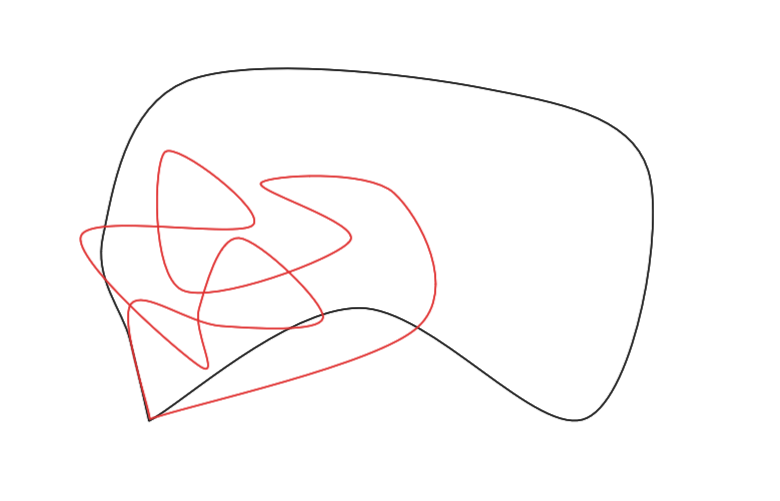
\includegraphics[width=0.8\textwidth]{bilder/CoveredAreaSketch.png}
		\caption{An example sketch showing the outlines of two different tours.}
		\label{fig:coveredAreaSketch}
	\end{centering}
\end{figure}

Figure \ref{fig:coveredAreaSketch} shows the outlines of two possible tours, where the black outline is more round than the red one. 
Here, the covered area of the black tour is larger than the one of the red tour, since in the calculation, all smaller areas are accounted for regarding their overlap as well as the direction of the turns (clockwise or counterclockwise).
Thus, the many overlaps of areas and the crossings of path parts reduce the covered area value.
Using this calculation, the red tour has a lower covered area, making the black one more desirable.



Tour4Me implements a solution for the \texttt{Touring Problem}, which is used to describe the task of finding appealing and ideally interesting roundtrips.
To achieve a relatively good solution, two factors are taken into consideration.
First is the total profit, that can be collected within the given length restriction for the tour.
The second factor is an additional quality function that assures for a relatively round tour by maximizing the area that is surrounded by the created roundtrip.
Tour4Me presents a selection of four different algorithms to calculate the tour as well as some additional customization options.
The offered choices include a Greedy Selection approach, Integer Linear Programming, MinCost with Waypoints, which are intermediate points used to calculate shortest paths between them (see \ref{subsubsec:runningRoutes} for more details), and Iterative Local Search (ILS) \cite{buchin_tour4me_2022}. 

The Greedy Selection \cite{buchin_tour4me_2022, wayahdi_greedy_2021} is the simplest algorithm out of the four and only ensures that the chosen route is a roundtrip.
The resulting path is built by iterating over the valid edges and picking the most profitable of these until the cycle is finished or no candidate is left.
A valid edge is determined by checking whether the start- and endpoint \textit{s} can still be reached if that selected edge is picked next. 
Edges that yield the highest profit and are valid are chosen at every node \cite{buchin_tour4me_2022, wayahdi_greedy_2021}.


For Integer Linear Programming \cite{buchin_tour4me_2022, graver_foundations_1975}, the \texttt{Touring Problem} must be stated in an appropriate form.
To do so, a single instance can be encoded as $\mathcal{I}(G, w, \pi, B, v_0)$, containing the Graph $G$, edge costs $w$, the profit function $\pi$, the budget (length restrictions) $B$, and the starting (and end-) point $v_0$.
Given this encoding, cycles $P=(v_0,...,v_i,...,v_0)$, which are always at most of length \textit{L}, can be built.
For the current definition, a few additional variables can be introduced to encode whether or not an edge is part of a solution (and how many times this edge occurs), whether or not an edge is the k-th edge of the solution, and whether or not a vertex is the k-th vertex of a solution. 
Using these variables, constraints can be built to describe the desired behavior of the algorithm.

The MinCost algorithm \cite{buchin_tour4me_2022, gemsa_efficient_2013} requires \textit{Waypoints} since the basic algorithm is designed to solve shortest path problems. 
Without these added Waypoints, the underlying computations would always result in never leaving the starting position. 
Even though this algorithm is not originally meant to solve roundtrip problems, the implementation takes into account the cost and profits of edges to create a solution tour, which makes this method more suited to the task than a simple Greedy search.
To create an optimized tour, the inefficiency of paths must be measured. 
This optimization is done by calculating the quotient of the edge costs and the profit the edge yields. 
Using this inefficiency, a ring of candidate points $R_s$ surrounding the starting point \textit{s} can be calculated.
From these candidates, new rings $R_r$ with the same requirements can be calculated. 
The solution path is then obtained by selecting all those circles that intersect with $R_s$.
In order to guarantee the best solution, all possible combinations are calculated and the most favorable of these solutions is returned \cite{buchin_tour4me_2022}.
Further details can be found in the original paper by Gemsa et al. \cite{gemsa_efficient_2013} which offers a Greedy Faces approach as well as two variants for the Partial Shortest Paths algorithm, of which the 2-via-routes option was implemented in Tour4Me.

Building on the solution that was constructed using MinCost, Iterative Local Search \cite{buchin_tour4me_2022, lu_arc_2015, verbeeck_extension_2014} can be applied to improve the found tours.
ILS is split into two main phases: the removal step and the improvement step.
The algorithm starts with a full roundtrip and then removes partial paths $P$ from the current best solution $S$ (the removal step).
After that, the previous tour now has a gap, which must be closed by iteratively adding new vertices and edges that improve the solution profit while always staying within the given budget (the improvement step).
When adding new edges to the solution that close the path, both the profit as well as the length of these paths must be considered. 
Since the roundtrip has a given maximum length, the profit must be maximized while keeping track of and never exceeding this length constraint.
The best solution is constantly improved until the user-selected time limit is reached.

Searching for viable edges is performed using a depth first approach.
Thus, bounding the maximum depth of this step can drastically speed up the algorithm.
This speedup then results in more iterations of removal and improvement being possible within the given time limit.



\subsection{Roundtrip Paths}
\label{subsec:Roudtrip}
There are a few tools and some research that deal with the construction of roundtrips.
Some of the papers specifically focus on running routes (\cite{gemsa_efficient_2013, pajor_algorithm_2013}) or tours tailored to cycling (\cite{ehrgott_bi-objective_2012, verbeeck_extension_2014}).
RouteLoops and RouteYou are two commercial tools that offer an interface to calculate tours, but do not have many customization options.
Neither has there been much research on roundtrip generation, nor are there any tools that offer customizability.
Aside from these few approaches for roundtrip calculation, some ideas to improve the experience and training effect of running, how to assist various different sports with technology, and even approaches on how to determine pleasant surroundings of paths have been developed, but these approaches have not been combined into a single application yet.



\subsubsection{Computing Running Routes}
\label{subsubsec:runningRoutes}

The problem of calculating good running roundtrips is not new.
In addition to the commercial applications, there are research papers on this subject as well.
One of these papers by Gemsa et al.\ \cite{gemsa_efficient_2013} presents two approaches to handle the new routing problem labeled \texttt{Jogging Problem} by the authors, which is split into two variants: 
one being the simple version that only aims to build a cycle containing the starting point \textit{s} and with the desired length.
The other variant is a more complex version that allows for some flexibility regarding the length of the final tour during optimization, which is named \texttt{Relaxed Jogging Problem} \cite{gemsa_efficient_2013}. 
This relaxation allows for considering more factors to also optimize for the resulting shape, the area surrounding the tour, and/or the simplicity of the path. 

The second problem is chosen as the one to optimize, since the relaxation enables the addition of conditions other than just the length of a tour.
For solving this selected problem, two different ideas are proposed.
The first approach -- \textit{Greedy Faces} -- is based on the idea of extending previous cycles.
The algorithm starts with a cycle containing the starting point \textit{s} that can be selected by the user. 
This roundtrip can then be extended to gradually approach the length specified by the user. 
The second algorithm is named \textit{Partial Shortest Paths} and uses Waypoints or \textit{Via-Vertices}.
These Waypoints are a number of new points that can be connected using shortest paths.
When the via-vertices are connected with each other and the start, they form a roundtrip.


For both algorithms, the authors measure the badness of paths, the number of edges that are shared, as well as the number of turns.
The badness is used to take the additional constraints into account. 
To reduce the possibility of having a roundtrip which turns at the end and uses all paths twice, the number of shared edges has to be minimized.
Otherwise, this construction would effectively form a simple U-turn tour (turning by 180 degrees).
The number of turns corresponds to the complexity of the tour and is measured by a percentage of doing a full U-turn. 
Gemsa et al.\ define the point between two edges as a \textit{turn} if the angle is larger than or equal to 15 degrees and less than 180 degrees.
These turns can then be used to determine the complexity of a tour:
More turns meaning a more complex tour.


%
%\paragraph{Greedy Faces}
%
%Greedy Faces is built from an already existing path by extending it.
%For this, blocks outside the given tour that are adjacent to the current path are used.
%The previous cycle then is changed so that it encloses the chosen block and thus extends the preceding route. 
%New blocks are picked until the desired length is reached.
%To ensure only blocks that correspond to faces are picked, a preprocessing phase is introduced that identifies faces of the graph.
%During this step, first, dead-ends are removed, so the resulting graph will be two-connected.
%Faces then are defined by the edges that surround them. 
%While identifying all faces, a dual graph $G^{\star} = (V^{\star},E^{\star})$ for $G = (V,E)$ is built as well.
%
%The Greedy Faces algorithm then works on the dual graph $G^{\star}$, selects a face \textit{f} from $V^{\star}$ which has a surrounding path that contains the starting point \textit{s}. 
%Then, a Breadth First Search Tree \textit{T} is built, starting at \textit{f}, until the desired length (a relaxed version $(1 + \varepsilon) L$) is exceeded.
%The resulting tour will be a simple path iff all vertices in \textit{V} without the ones in \textit{T} are connected and contain \textit{s}.
%The final jogging path can be extracted by taking the cut edges between the tree \textit{T} and the remaining vertices.
%This always forms a cycle and thus builds a roundtrip.
%
%For building a path which optimizes all constraints, the three introduced measures for badness, number of shared edges and the number of turns are used.
%The badness function is incorporated into a different force function $\varphi (f,p) = \frac{(\text{bad}(f)-0.5)l(f)}{|\vec{d}|^2} \cdot \frac{\vec{d}}{|\vec{d}|}$ which can assign positive and negative badness values to edges.
%Furthermore, the force function uses the cost of the face and a vector $\vec{d} = \vec{p} - \vec{C}(f)$ which is built from the geometric center $\vec{C}(f)$ of a face to any point $\vec{p}$. 
%This force vector can then be used to calculate the best next edge for extending the current path by maximizing $\varphi(g) cos (\measuredangle (\varphi(g), C(f) - C(P)))$, measuring the angle between the directed force vector and the geometric center point \textit{C(P)} of the path that has been built so far.
%The force vector is used in the Breadth First Search but it doesn't have to be the only criteria.
%An extension to include other measures like roundness or complexity can be created as well. \cite{gemsa_efficient_2013}
%
%
%After the tour has been created, it will be smoothed to reduce the complexity.
%This is done by building a subset (always including \textit{s}) of the nodes contained in the created path and computing shortest paths between all vertex pairs in this subset. 
%Concatenating them will then return a smoothed path.
%This approach is extended to again take badness into account as to not create a bad final path because of the smoothing step. \cite{gemsa_efficient_2013}
%
%The Greedy faces algorithm does extend an initial cycle, but it has no guarantees on the length of the final returned path.
%It can deviate without constraints from the original user specification, resulting in paths that can be way too short or way too long. \cite{gemsa_efficient_2013}
%
%
%\paragraph{Partial Shortest Paths}
%
%Since Greedy Faces cannot give any guarantees, the authors pursued a second approach to calculating results that are ensured to deviate at most by a small $\varepsilon$.
%The partial shortest paths are based on a set of via-vertices and named by the number of intermediate points created. 
%In the paper, 2-via-routes and 3-via-routes are presented.
%
%For two intermediate points, three shortest paths have to be calculated.
%These furthermore have to have a length of $\frac{1}{3} L \pm \varepsilon$, building a triangle.
%Again, the shortest path calculation used will also consider the badness of the edges when selecting them.
%Optimizing this metric will return a set of feasible candidate paths that are \enquote{nice} - as the authors describe this property - and create a ring around the starting point.
%
%From this point, another ring with a diameter of $\frac{1}{3} L \pm \varepsilon$ is calculated from every vertex within the first ring.
%All elements that are within the intersection of both rings are valid candidates for the third point to be selected. 
%The final path is created by picking the tour with a minimal badness from all feasible combinations of \textit{s} and the two other selected vertices. \cite{gemsa_efficient_2013}
%
%The three point variant 3-via-routes is an extension to improve the smoothness around the two selected vertices for building the initial triangle. 
%The algorithm then builds the ring around the starting point as in the first version but with a narrower radius of $\frac{1}{4} L \pm \varepsilon$.
%Then, an even narrower ring is created, using a new parameter $\alpha \in [0.5,1]$ as a condition for the radius of the new ring: $\frac{\alpha}{3} L \pm \varepsilon$.
%The value of $\alpha$ and a new point \textit{m} in the middle of the created path control the smoothness around the two other vertices.
%
%From the two triangle points \textit{u} and \textit{v}, new points \textit{u'} and \textit{v'} within the narrower ring are obtained by following the shortest path trees. 
%Then, new rings around these vertices are calculated, using a radius of  $\frac{2-\alpha}{4} L \pm \varepsilon$ to ensure a distance of  $\frac{1}{2} L \pm \varepsilon$ for all vertices within each of these rings.
%This results in a ring containing possible middle vertices.
%Then, for all pairs \textit{u'} and \textit{v'}, the intersection of their respective rings can be built and all middle vertices that will yield a smooth path for the two triangle points \textit{u} and \textit{v} will be selected as middle point candidates.
%Finally, the path along the vertices that has minimum badness will be returned as the result. \cite{gemsa_efficient_2013, pajor_algorithm_2013}
%
%Both, the Greedy Faces as well as the Partial Shortest Paths offer a solution to the roundtrip problem.
%They also allow for customization of the tour using different constraints. 
%This is why the Partial Shortest Paths approach is already used as one available option in Tour4Me. 
%The constraints and parameters that can be used to influence properties of the tour offer fewer customization options than it is planned for this thesis. \# TODO do I have to specify what is different from my approach for every paper I mention here?


\subsubsection{Computing Cycling Routes}
\label{subsubsec:cyclingRoutes}

For cycling, there are some papers (\cite{ehrgott_bi-objective_2012, verbeeck_extension_2014}) discussing ideas for generating cycling tours.
Ehrgott et al.\ \cite{ehrgott_bi-objective_2012}  discuss a bi-objective model that takes travel time and \textit{suitability for cycling} into account.
Suitability is defined as a combined measure of objective factors, containing but not limited to the volume and speed of traffic on the roads, which can impact the safety of these path segments. 
However, subjective values like the individual fitness level are not considered for this implementation.
All objective values that are regarded significant for the suitability of the tour are accumulated into this single measure, so that there are only two values to optimize at the same time. 

The authors offer a solution for the issue that many of the values can have a different level of importance for different people. 
While some people might not want hilly routes at all, others could enjoy the challenge a certain steepness presents. 
Because of this difference in basic preferences, Ehrgott et al.\ chose to offer a choice set of several alternative routes, from which the user can pick the one that works best with their personal preferences. 

This approach takes several different factors into account, but does not offer any means to influence the importance specific factors have on the generated routes beforehand.
Furthermore, the presented ideas are focused on shortest path applications, not on roundtrips.

Verbeeck et al.\ \cite{verbeeck_extension_2014} concentrate on cycle trips in their paper, which also builds a foundation for the ILS algorithm used in Tour4Me (see Section \ref{subsec:Tour4Me}). 
The authors build a \texttt{cycle trip planning problem (CTPP)} as an alternative version of the Arc Orienteering Problem (see Section \ref{sec:aop} for further details). 
The initial idea is to use a metaheuristic approach of ILS to build roundtrips that optimize the profit of the trip.
Since the AOP is already NP-hard and the CTPP has an even higher complexity, attempting to solve this problem with an analytic, exact algorithm will not be feasible in terms of time constraints. 
Because of this complexity, the authors developed two approaches -- a branch-and-cut algorithm and a metaheuristic method -- to try and solve their CTPP quickly. 
The branch-and-cut approach turned out to return results on smaller sets within a reasonable time.
However, the algorithm is too slow for larger problem space instances.

Therefore, Verbeeck et al.\ developed the ILS approach which can be split up into three phases:
initialization, improvement, and selection.
During the initialization phase the implemented algorithm gathers a first set of possible solutions by using the insert move that aims to find a path with the highest score.
The insertion phase starts with every arc that leaves the starting point and builds a maximum-profit path until a feasible solution is obtained.
This step is done for all possible starting points, so several solutions are created.
Then, the results from the previous step are optimized in the improvement phase. 
To do so, a part of the solution is removed during every iteration.
Next, the newly constructed gap between the two nodes where the path was removed is closed, using the same insert move from the initialization, thus improving the previous solution.
This process then iterates over the whole tour until the removal encounters the end vertex (which is equivalent to the start vertex) again.

Using this approach, the authors were able to create a path within the given time constraints, build a roundtrip, ensure that its length lies between a maximum and minimum value and optimize its profit.
They also stated that their ideas can be used as \enquote{building blocks}  \cite{verbeeck_extension_2014} for further development.
The fact that Verbeeck et al.\ stress, is that vertices can be visited multiple times (except the start vertex), however arcs and their complements (if existent) cannot. 
Thus, they enforce trips to not take the same paths twice.

They conducted several benchmark tests for their implementations, but the code is not publicly available.
Furthermore, there does not seem to be any way to try out the existing implementation and assess how many parameters are used, which of them can be changed and how much customization is overall possible.
The fact that the authors do not allow passing an arc twice also limits the options to select a preferred tour shape that might include those that simply run one way and have a U-turn at the end. 


\subsubsection{RouteLoops \& RouteYou}
\label{subsubsec:routeLoopsrouteYou}

RouteLoops and RouteYou are two commercial programs that can be found and used online. 
However, neither the code itself nor information about the implementation are accessible.

RouteLoops has two text fields for entering the starting point and the length of the trip.
Aside from that, no customization is possible.
The interface has a few features to show more information about the route.
After the calculation, distance markers or elevation can be displayed.
However, these outputs cannot be used as inputs to get a route with as little elevation as possible.
The page claims that the difficulty of a route can be shown for tours that are placed within the United States.
However, even when creating a route in the United States, a display of the difficulty could not be replicated. 
RouteLoops also does not actually create loops but rather picks a route that has a high value (for example with a river in a park) and lets the user run along that path, turn around at the end and run back the same way.

To create a roundtrip, some Waypoints are used. 
These points can be removed or more can be added when editing the tour.
Between the Waypoints, the shortest path is created to connect them. 

RouteYou offers several different user input options that will return varying results, however, picking the same option again will also give different results every time.   
Here, the roundtrips are more round than with RouteLoops, but again, elevation or difficulty are not taken into account. 
Even though both do offer the possibility to edit the returned roundtrip, this editing changes the length of the route arbitrarily.
Furthermore, the user cannot specify directly what type of surface, surroundings, etc. are preferred. 




\subsection{Other Running Related Research}
\label{subsec:otherRunningResearch}

Aside from the few directly related papers and applications, some general research regarding running with technology has been done.
Jensen and Mueller \cite{jensen_running_2014} focus on the utilization of interactive technologies that can be used to monitor or enhance the performance of athletes.
They are particularly interested in improving these gadgets and apps to enhance their usability. 
In their paper, they discuss the current state of different technologies and propose the following three key questions as ideas of what aspects to focus on for further improvement:
The first question \enquote{How to interact} focuses mainly on the question how interaction with any app or gadget can be designed so it will not hinder the actual activity of running.
The second question \enquote{What information} aims to enhance the types of information presented to the user while running (for example to change the running style mid-run)
While the third question \enquote{When to assist} addresses the timing aspect of any kind of assistance during a workout. 
They strive to find suggestions on what to focus on when trying to produce apps or gear for runners.



\subsection{Apps That Assist with Sports}
\label{subsec:runningApps}

Aside from Tour4Me, RouteLoops and RouteYou, another prototype for running route recommendations has been developed.
Other papers, such as one by Loepp and Ziegler \cite{loepp_recommending_2018}, used the Partial Shortest Paths algorithm from the idea Gemsa et al.\ presented \cite{gemsa_efficient_2013} to build a recommendation-based app.
However, they tried to incorporate more criteria, such as elevation levels or information about the surroundings, allowing users to pick from a variety of options when generating personalized tours. 
Furthermore, the authors added a feature to use routes by other users, but their subsequent survey revealed that none of their users were interested in that particular feature.

The customized tours that could be generated were well-received, perceived as high-quality, and the difficulty was considered low by the users.
This app is only a prototype and was never fully expanded into a full-fledged product.
Currently, the app runs only on smartphones that use Android. 

In the corresponding paper \cite{loepp_recommending_2018}, Loepp and Ziegler also express several issues with and shortcomings of existing apps.
Some of these problems have already been identified in the introduction of the two websites RouteLoops and RouteYou (see \ref{subsubsec:routeLoopsrouteYou}).
They also stress that most research either concentrates on shortest paths or on the assistance with the training itself rather than finding a good route.

Apps like \textit{Runtastic}\footnote{\url{https://www.runtastic.com/}, last accessed: 22.03.2024}, \textit{Sportractive}\footnote{\url{http://sportractive.com/}, last accessed: 22.03.2024} or \textit{Strava}\footnote{\url{https://www.strava.com}, last accessed: 22.03.2024} are designed to help runners track the tours they have already run. 
These apps measure pace, position, altitude, and several other stats during a run, to then provide feedback to the user. 
Planning a route is not one of the features these apps offer.
Even apps designed to assist with the training and creating a plan such as \textit{Trainingpeaks}\footnote{\url{https://www.trainingpeaks.com/}, last accessed: 22.03.2024} or \textit{SportTracks}\footnote{\url{https://sporttracks.mobi/}, last accessed: 22.03.2024} do not offer a feature to create routes or roundtrips based on a set of preferences \cite{loepp_recommending_2018}.

A German app that is meant to provide suitable routes for a variety of different outdoor sports \textit{Komoot}\footnote{\url{https://www.komoot.de/}, last accessed: 22.03.2024} does offer a route selection. 
However, only tours other users have planned manually and added can be selected. 
No customization or automated route creation is offered. 
As Loepp and Ziegler pointed out in their user study \cite{loepp_recommending_2018}, user feedback, their preferences, and the option to customize were crucial features for a route generation app. 
%The fact that no participant in their study chose to try out a route recorded by another member further stresses the importance of personalized route generation.


\subsection{Other tour optimization ideas}
\label{subsec:otherTourOptimization}

Aside from approaches to calculate good roundtrips and the various sports-assisting apps and technology, there is another point that is related to generating desirable tours.
Some papers (e.g. \cite{alivand_analyzing_2015}) discuss the question of how to find scenic routes, which aspects impact how appealing a route is, and how the availability of more panoramic routes can influence the users' decisions.
To gain some understanding of what is considered scenic and what features can lead users to take longer tours into account, Alivand et al.\ \cite{alivand_analyzing_2015} created a route choice model.
Their application calculated and displayed the shortest path from a source to a destination and additionally a set of routes that were longer (considering their length or the travel-time or both) but had more panoramic views along the path.
The points they used to decide what can be considered a scenic view were gathered from a set of geo-tagged photos and travel blogs.

From their testings, users were happy to take detours that were on average 90\% longer than the fastest tour.
%This observation shows how important the view and surroundings can be when the goal is not necessarily to find a quick or short path, but also to take other subjective parameters into account.
The paper focused on touristic trips from a start to a specific destination, but their findings can easily be translated to other modes of travel, including roundtrips.





\section{Goal and Methodology}
\label{sec:goal}

As stated before, existing tools that can calculate roundtrips leave out certain data like the elevation of nodes or path types of edges.
The absence of these information impacts the quality of the created routes for individual users or even whole user groups. 
For example, people who prefer running with little to no elevation might end up with a route that takes them uphill for half of the distance.
While this path may be a suitable choice for other users -- such as joggers who prefer more challenging routes or those who want to hike and enjoy ascending -- the constant elevation gain can be undesirable for beginners.
Some people might prefer to choose whether they are running through the city or in a park depending on the elevation level.
For these users, the created route would be highly unfavorable, even though the result matches other constraints for what is considered a nice roundtrip.
Therefore, giving the user as many customization options as possible without becoming overwhelming can be a crucial point. 


The goal of this thesis is to develop a usable application for computing running or cycling roundtrips of (almost) arbitrary length. 
In this context \textit{usable} means an app that operates in real-time, produces routes of the desired length, and prioritizes paths based on the user's input. 
To achieve this goal, this thesis is an extension of the already existing prototype Tour4Me \cite{buchin_tour4me_2022} and adds metaheuristic approaches that have been considered the most fitting for this purpose. 

First, an interface for testing the new approaches was built. 
To add user options like the length of the desired roundtrip, as well as other preference inputs, an additional overlay was needed.
Based on this interface, different algorithms were added and compared with each other to identify the ones that produced promising outputs.\footnote{\url{https://github.com/LisaSalewsky/MA-Customizable-Roundtrips-with-Tour4Me}, last accessed: 13.07.2024} 
However, the definitions of a high quality result can vary significantly based on the criteria used. 
An ideal algorithm would be fast, consistently generate a route, and incorporate all user preferences.
Achieving all these objectives with a single algorithm is not possible. 
Therefore, various approaches have been implemented and analyzed according to how well they meet the mentioned criteria. 

The implemented approaches include Ant Colony \cite{babaoglu_anthill_2002, dorigo_ant_1996, gendreau_handbook_2010, wang_application_2014} and Simulated Annealing \cite{aarts_simulated_2005, delahaye_simulated_2019, eglese_simulated_1990, zhan_list-based_2016}.
Both of these metaheuristics have been implemented as a standalone solution as well as in combination with the previous Greedy algorithm, the MinCost implementation, and with each other.
After implementing the algorithms, the most suitable algorithms as well as the most fitting parameter configurations for Ant Colony, Simulated Annealing and the other variations had to be determined. 
The aim for the app was to calculate a high-quality tour for any typical roundtrip request for running and cycling.

In addition to finding suitable algorithms that allow for fast and reliable computation of all typical roundtrips, working on the interface and data used also enhanced the usefulness of the app.
Improving the interface and adding more options like elevation data, including more information (for example surrounding tags) have been equally important changes to increase the usability.
There are several opportunities to improve the app not only by changing the used algorithms but also through adding user selection options and upgrading the GUI.
Enhancing the interface through extending available inputs and sliders to better specify tour parameters, and overall refining the usability constitutes another pillar of improving the app aside from adding more or faster algorithms.

Overall, the goal of this thesis is to build a user-friendly application that can compute roundtrips for various outdoor activities.
This thesis focuses primarily on adding customization options and the respective front-end changes as well as the implementation of Ant Colony and Simulated Annealing as two metaheuristic approaches for solving the problem.
The resulting web application is able to calculate tours for (almost) any length, take user preferences into account, and operate in real time.








\section{Structure}
\label{sec:structure}

The second chapter covers the essential background information and fundamentals.
First, a brief overview of shortest path algorithms and the existing options is presented.
Afterwards, the Arc Orienteering Problem, which builds the basis for calculating paths that optimize for other values than their respective length, is presented and described in detail.
Then, the fundamentals of the two implemented algorithms Ant Colony and Simulated Annealing are explained.

Chapter three outlines the implemented changes, beginning with the overall architecture of the software and a list of the technologies and languages used.
Then the added database and data acquisition, as well as the needed processing are described.
Afterwards, the front-end changes, and new parameters are explained.
The final section of the third chapter gives of about the implemented algorithms and specifies where changes to the algorithms presented int the given literature were needed.
Furthermore, the implemented combinations are described.

In the fourth chapter, several test cases are conducted, and their results presented and analyzed.
Several parameter configurations for both implemented base algorithms had to be determined.
The effect of the customization options were also examined and displayed. 
Lastly, the chapter compares all implemented algorithms, noting their quality change over time.

The last chapter summarizes all results, detailing how the set goals were met.
The chapter concludes with several ideas for future work, highlighting potential areas for further development and optimization.








